\documentclass[12pt,letter]{article}
\usepackage[moduleName=Jairasullator]{KautenjaDSP}
\begin{document}
\titlePage{img/Logo}{img/Module}{img/KautenjaDSP}

% -------------------
% MARK: Overview
% -------------------

\section{Overview}

Jairasullator is an emulation of the General Instrument AY-3-8910 sound chip from many Arcade games. The AY features three tone generators, each with an optional noise effect. Jairasullator provides the key features of the General Instrument AY-3-8910 chip, namely,
\begin{itemize}
  \item \textbf{Triple pulse wave generator:} Three pulse waves with $50\%$ pulse width and 12-bit frequency value
  \item \textbf{Noise generator:} Generate pitched noise from each voice using the global noise generator with $32$ different frequencies
  \item \textbf{Tone/Noise control:} CV and switch to control tone and noise for each voice
  \item \textbf{4-bit Amplifier:} A 4-bit amplifier controls the output level of each voice with base/attenuator knobs and CV inputs
  \item \textbf{Envelope Generator:} Generate an envelope for each voice using the global envelope generator with eight different modes
  \item \textbf{Low Frequency Oscillator:} Generate low-frequency oscillations from each voice using the global envelope generator
  \item \textbf{DAC Emulator:} Optionally use each voice as a 4-bit DAC emulator with amplitude and bias control
  \item \textbf{Channel Mixer:} Mix the voices together internally with hard clipping and intentional aliasing
\end{itemize}

% -------------------
% MARK: Panel Layout
% -------------------

\clearpage
\section{Panel Layout}

\begin{figure}[!htp]
\centering
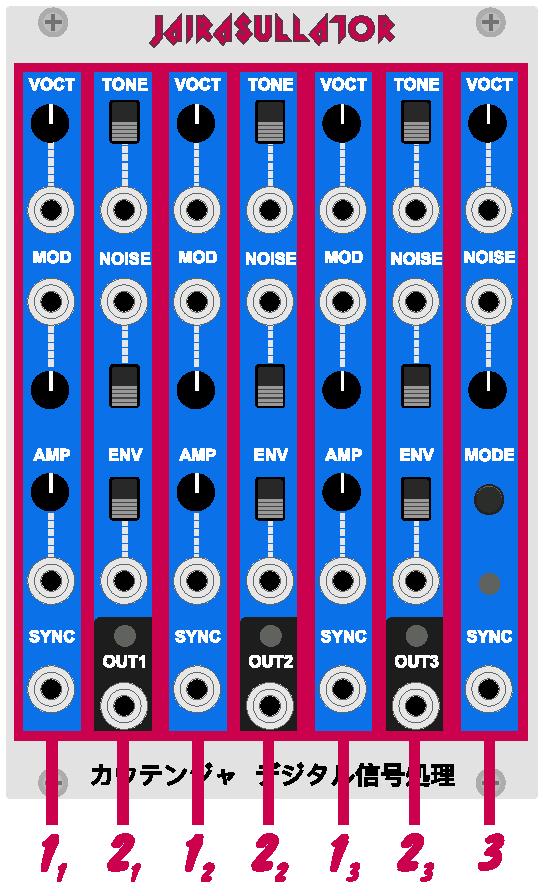
\includegraphics{img/Interface}
\end{figure}

% \begin{enumerate}
%   \item Coarse frequency control over the four oscillators. The frequency of oscillator 3 also controls the period of the noise generator.
%   \item $V$/Octave inputs for tone1, tone2, and tone3 waveform generators.
%   \item linear CV frequency modulation for tone1, tone2, and tone3 waveform generators.
%   \item On/off control over pulse generator (top) and noise generator (bottom) for each oscillator. The CV gate input goes high at $2V$. The toggle switch both acts as a basic switch and inverts the effect of the CV gate input.
%   \item Coarse amplitude control over the oscillators using the 4-bit amplifier.When no input is connected, the slider controls the level from $0\%$ to $100\%$. When an input is connected, the slider acts as an attenuator.
%   \item Channel outputs, ${\approx}10V_{pp}$.
% \end{enumerate}

\subsection{Voice Control}

The \textbf{VOCT} trimpot controls the coarse frequency of the three pulse waveform generators. Frequency is quantized to a 12-bit value for the oscillators, which is particularly noticeable in the very low / high registers. The \textbf{VOCT} ports provide an exponential $V$/Octave input for controlling the pitch of the tone generators. Inputs are normalled forward from Voice 1, to Voice 2, to Voice 3, to the Envelope Generator.

The When nothing is patched to the \textbf{MOD} port, the trimpot can be used to fine tune the frequency of the given waveform generator. When a signal is patched, the \textbf{MOD} port provides linear frequency modulation to the corresponding waveform generator and the trimpot can be used as an attenuverter to attenuate / polarize the incoming signal. Inputs are normalled forward from Voice 1, to Voice 2, to Voice 3, and support audio rates.

When no input is connected, the \textbf{AMP} trimpot controls the given waveform generator volume level with 4-bit resolution (i.e., $\in [0, 15]$). When an input is patched to the \textbf{AMP} port, the trimpot acts like an attenuator that scales the CV control over the volume level. Because the amplifier has 4-bit control, the envelope of the voice will sound quantized when used with an external envelope generator. Inputs are normalled forward from Tone 1, to Tone 2, to Tone 3, and support audio rates.

When a voice is in DAC mode (Tone, Noise, and Envelope are all off), the \textbf{AMP} port acts as an audio rate signal input to the DAC. The \textbf{VOCT} parameter acts like an offset control for adding DC offset to the incoming signal. This control is necessary to turn the AC signal into a DC signal for the chip to process. The \textbf{MOD} parameter acts as a attenuator for controlling the amplitude of the incoming audio signal. The \textbf{AMP} trimpot controls the ouput level of the voice.

The \textbf{SYNC} input can be used to hard sync the pulse waveform generator to another oscillator. The sync port supports audio rate modulation.

\subsection{Voice Mode}

When the \textbf{TONE} switch is pointing up, the given voice's tone generator is enabled. When pointing down, the tone generator is disabled for the voice. The \textbf{Tone} input port acts like a gate that goes high at $2V$ and inverts the value of the \textbf{TONE} switch.

When the \textbf{NOISE} switch is pointing up, the given voice emits sound from the global noise generator. When pointing down, the noise generator is muted for the voice. The \textbf{NOISE} input port acts like a gate that goes high at $2V$ and inverts the value of the \textbf{NOISE} switch.

When the \textbf{ENV} switch is pointing up, the global envelope generator is enabled for the voice. When pointing down, the noise generator is disabled for the voice. The \textbf{ENV} input port acts like a gate that goes high at $2V$ and inverts the value of the \textbf{ENV} switch. The envelope generator can be used to envelope a voice when tone and/or noise are enabled, or it can be used as a global LFO when both tone and noise are disabled for the voice.

Each voice produces an output signal of at most $10V_{pp}$ when the amplifier is maxed out. The individual oscillators cannot be overdriven to produce clipping, distortion, or aliasing. However, outputs are normalled forward into a sum mix where hard clipping \textit{can} occur. Excess clipping will introduce an aliasing effect to the mix. Outputs in the mix are clipped \textit{before} being normalled to the next output. VU meter lights measure the output of individual channels going from off ($-\infty dB$ to $-12dB$), to green ($-12dB$ to $0dB$), and lastly to red ($0dB$ to $3dB$) when clipping begins to occur\footnote{This includes LFO modes}.

\subsection{Envelope and Noise Generator}

The \textbf{VOCT} trimpot controls the coarse frequency of the global envelope generator. Frequency is quantized to a 16-bit value, which is particularly noticeable in the very low / high registers. The \textbf{VOCT} port provide an exponential $V$/Octave input for controlling the pitch of the envelope generator. When nothing is patched to the \textbf{VOCT} port, the signal from port 3 is normalled as the input.

The \textbf{NOISE} trimpot controls the pitch of the global white noise generator for the module $\in [0, 31]$. When an input is patched to the \textbf{NOISE} port, the trimpot acts as a bias control and the CV offsets the parameter in increments of $250mV$.

The \textbf{MODE} button cycles between the 8 modes of the envelope generator listed by Table~\ref{tab:envelope-generator}. The LED provides an indication of the current mode.

\begin{table}[!htp]
\centering
\caption{The modes of the envelope generator.}
\label{tab:envelope-generator}
\begin{tabular}{|c|l|c|}
\hline
 \bfseries Color                                          & \bfseries Mode   & \bfseries Envelope Shape                      \\
\hline\hline
 \tikz\draw[black,fill=black] (0,0) circle (1ex);         & Attack           & 
\includegraphics{img/Envelope/Attack}         \\
\hline
 \tikz\draw[black,fill=blue!70!white] (0,0) circle (1ex); & Decay            & 
\includegraphics{img/Envelope/Decay}          \\
\hline
 \tikz\draw[black,fill=green!60!white] (0,0) circle (1ex);         & Attack and Max   & 
\includegraphics{img/Envelope/AttackMax}      \\
\hline
 \tikz\draw[black,fill=blue!20!white] (0,0) circle (1ex); & Decay and Max    & 
\includegraphics{img/Envelope/DecayMax}       \\
\hline
 \tikz\draw[black,fill=red] (0,0) circle (1ex);           & Attack LFO       & 
\includegraphics{img/Envelope/AttackLFO}      \\
\hline
 \tikz\draw[black,fill=pink] (0,0) circle (1ex);          & Decay LFO        & 
\includegraphics{img/Envelope/DecayLFO}       \\
\hline
 \tikz\draw[black,fill=yellow] (0,0) circle (1ex);        & Attack-Decay LFO & 
\includegraphics{img/Envelope/AttackDecayLFO} \\
\hline
 \tikz\draw[black,fill=white] (0,0) circle (1ex);         & Decay-Attack LFO & 
\includegraphics{img/Envelope/DecayAttackLFO} \\
\hline
\end{tabular}
\end{table}

The \textbf{SYNC} input can be used to hard sync the envelope generator in LFO mode, or to trigger it in one-shot mode. The sync port supports audio rate modulation.

% -------------------
% MARK: References
% -------------------

\clearpage
\renewcommand\refname{References}
\nocite{*}
\bibliographystyle{apalike}
\bibliography{references}

\end{document}
